\documentclass[11pt]{article}
\usepackage[margin=2.5cm]{geometry}\usepackage{amsmath,amssymb,graphicx,listings,hyperref}
\lstset{basicstyle=\ttfamily\footnotesize,breaklines=true,frame=single}
\title{A Discrete Model for the Performance of a Filter-Based Air Purifier in a Closed Room}
\author{Ray Parker}\date{}
\begin{document}\maketitle
\begin{abstract}
A step-by-step model for how a filter-based purifier lowers pollutant levels in a closed room of nearly constant air volume. Pollutants are treated as a solute in the air (the solvent). The note sets out the model as written on the original handwritten page, states the range where it holds, gives a refinement, and compares both with the standard clean-air-delivery-rate (CADR) exponential decay in an illustrative simulation.
\end{abstract}

\section{Setup and definitions}
The room is closed (somewhat isolated) with nearly constant air volume. Pollutants are treated as solute particles in the air, which acts as solvent. Define
\[ S_t=\frac{\text{amount of solute per unit volume}}{\text{amount of solvent per unit volume}}\quad\text{at time step } t. \]
Other quantities:
\begin{itemize}
\item $\mathrm{Vol}_t$: volume passed through the filter at step $t$ (starting just after $t-1$), with $\mathrm{Vol}_t=\mathrm{Vol}_0\,c(t-1)$, where $c(t)$ is the filter clog factor at time $t$;
\item $x_t$: solvent per volume at time $t$;
\item $\gamma$: an allowance factor that makes the filter realistic;
\item $\mathrm{Sol}_0$: amount of solute at time $0$;
\item $\alpha_t$: amount of solute removed at step $t$.
\end{itemize}

\section{The model}
\begin{equation}\label{eq:main}
S_t=S_{t-1}\left(1-\frac{\alpha_{t-1}}{\mathrm{Sol}_0-(t-1)\,\alpha_0}\right),\qquad t\ge1,
\end{equation}
with $S_0=S_{-1}=S_{-2}=\cdots$ by definition. The removal is
\begin{equation}\label{eq:alpha}
\alpha_0 \;\text{measured at the start (a fixed input)},\qquad
\alpha_t=S_t\,\mathrm{Vol}_t\,x_t\,\gamma\quad(t\ge1).
\end{equation}
So the first-step removal $\alpha_0$ is nonzero and measured, not computed; every later step follows the formula.

\paragraph{Reading the recurrence.} The fraction $\alpha_{t-1}/(\cdot)$ is the share of the solute still present that the filter removes in one step, and $S$ drops by that share. The denominator estimates the remaining solute by assuming each earlier step removed the same amount $\alpha_0$.

\paragraph{Range of validity.} The denominator reaches zero when $(t-1)\alpha_0=\mathrm{Sol}_0$, so the model holds for
\[ t<\frac{\mathrm{Sol}_0}{\alpha_0}+1. \]
Since later steps remove less than $\alpha_0$ (cleaner air, more clogging), the constant-$\alpha_0$ estimate of what is left is too low, so the model decays somewhat faster than reality as $t$ nears this limit. Early on it is accurate.

\section{Refinement: exact remaining solute}
Replacing the estimate with the solute actually left before step $t-1$,
\begin{equation}\label{eq:ref}
S_t=S_{t-1}\left(1-\frac{\alpha_{t-1}}{\mathrm{Sol}_0-\sum_{k=0}^{t-2}\alpha_k}\right),
\end{equation}
removes the singularity. (The sum has $t-1$ terms, matching the $(t-1)\alpha_0$ it replaces; if all $\alpha_k=\alpha_0$ the two agree.) If the remaining solute is proportional to $S_{t-1}$, the ratio becomes $\mathrm{Vol}_{t-1}x\gamma/(\text{room solvent})$, a per-step removal fraction that shrinks only through clogging.

\section{Link to CADR decay}
For a well-mixed room of volume $V$ and a purifier with clean air delivery rate CADR, $C(t)=C_0e^{-\mathrm{CADR}\,t/V}$. With no clogging ($c\equiv1$) and constant $x$, the refinement removes a constant fraction $f$ each step, so $S_t=S_0(1-f)^t\approx S_0e^{-ft}$: the discrete CADR law with $f=\mathrm{CADR}\,\Delta t/V$. The clog factor $c$ turns the constant rate into a slowly falling one, and $\gamma$ accounts for imperfect capture.

\section{Illustrative simulation}
Parameters are \textbf{illustrative only, not measured}: $S_0=1$, $\mathrm{Sol}_0=100$, $\alpha_0=5$, $\mathrm{Vol}_0=10$, $x=1$, $c(s)=e^{-0.02\max(s,0)}$, and $\gamma=0.5$ (chosen so the formula would give $\alpha_0$ at $t=0$). The exponential uses $f=\alpha_0/\mathrm{Sol}_0=0.05$ with no clogging. Validity limit: $t<21$.

\begin{figure}[h]\centering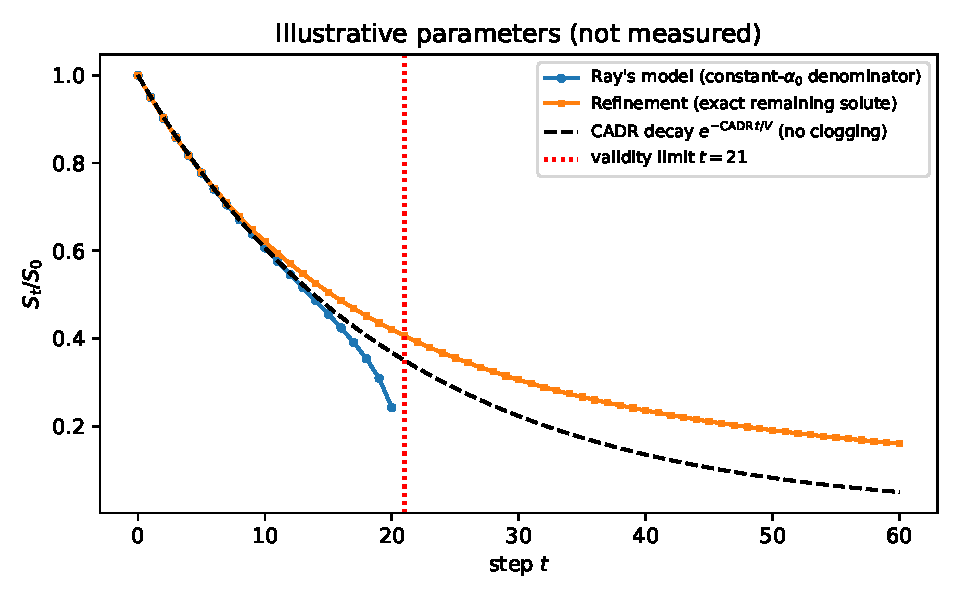
\includegraphics[width=0.85\textwidth]{simulation.pdf}
\caption{$S_t/S_0$ for the model, the refinement, and CADR decay (illustrative parameters).}\end{figure}

\begin{center}\begin{tabular}{lccc}\hline
step & model \eqref{eq:main} & refinement \eqref{eq:ref} & $e^{-0.05t}$\\\hline
$t=10$ & 0.607 & 0.621 & 0.607\\
$t=20$ & 0.243 & 0.420 & 0.368\\
$t=60$ & (outside range) & 0.160 & 0.050\\\hline
\end{tabular}\end{center}
Up to $t\approx10$ the model matches CADR decay closely. Near the limit it falls fastest, as expected. The refinement decays more slowly than the exponential because clogging reduces the flow.

\section{Code}
\lstinputlisting[language=Python]{simulate.py}

\appendix\section{Original handwritten page}
\begin{center}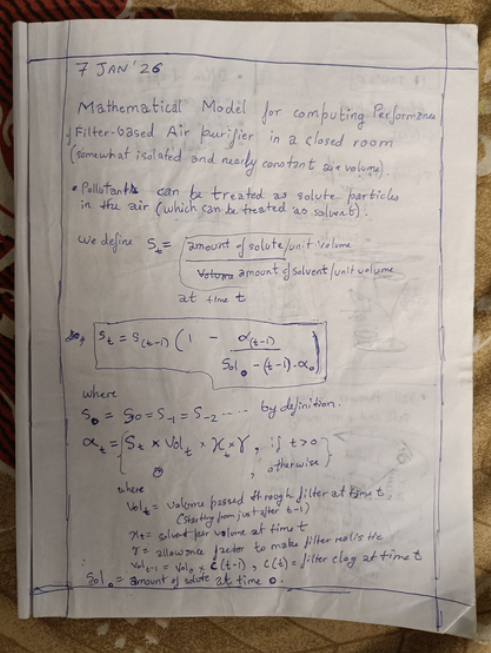
\includegraphics[width=0.6\textwidth]{notes-page.png}\end{center}
The page is a rewritten copy made to explain the approach.
\end{document}
